\documentclass[aspectratio=169]{beamer}
\usetheme{Warsaw}
\usepackage[utf8]{inputenc}
\usepackage[english]{babel}
\usepackage{amsmath}
\usepackage{amsfonts}
\usepackage{amssymb}
\usepackage{graphicx}
\usepackage{color, colortbl}
\usepackage{xcolor}
\usepackage{tikz}
\usetikzlibrary{
	arrows,
	automata,
        shadings,
        shadows,
        shapes,
}

\usepackage{pgfplots}
\usepackage{fontspec}
\newfontfamily\cjkfont{Noto Serif SC Black} % Or any appropriate font you have

\input{global_color_scheme.tex}
\input{tikz_process_steps/contsts.tex}

\author{leviathanch | chipforge | foshardware \ (Lanceville Technology)}
\title{Breaking the microchip monopoly}
\setbeamercovered{transparent} 
\setbeamertemplate{navigation symbols}{} 
%\institute{} 
%\date{} 
\subject{A free semiconductor manufacturing standard}
\begin{document}

%\begin{frame}
%\tableofcontents
%\end{frame}

\section[Standard Cells]{}
\begin{frame}{Standard Cells}
\end{frame}

\section[Silicon Compiler]{}
\begin{frame}{Open Source Tools}
	\begin{itemize}
        \setlength\itemsep{1em}
		\item yosys
		\item graywolf
		\item qrouter
		\item several FPGA routers
	\end{itemize}
\end{frame}

\begin{frame}{graywolf}
	\begin{itemize}
        \setlength\itemsep{1em}
		\item Originates in Academia: TimberWolf
		\item Simulated annealing
	        \begin{itemize}
		    \item Meta heuristic that is useful not only for placement
	        \end{itemize}
		\item Inline syscalls
	        \begin{itemize}
		    \item This is just a bad idea
	        \end{itemize}
	\end{itemize}
\end{frame}

\begin{frame}{qrouter}
	\begin{itemize}
        \setlength\itemsep{1em}
		\item Started in 2011 by Tim Edwards 
		\item Widely used for FPGA
	        \begin{itemize}
		    \item Not ready for silicon
	        \end{itemize}
		\item Sequential routing
	        \begin{itemize}
		    \item Parallelism not in scope
	        \end{itemize}
		\item Difficult to prove formal correctness
	        \begin{itemize}
		    \item Prove that C implementation of Rip-up and Re-route is correct
	        \end{itemize}
	\end{itemize}
\end{frame}

\begin{frame}{Productive Tools}
	\begin{itemize}
        \setlength\itemsep{1em}
		\item Different tool sets like BonnRoute, Cadence Suite, Alliance tools, etc.
		\item Similar capabilities with respect to silicon
		\item Just throw man-power at VLSI --- what is automation?
	\end{itemize}
\end{frame}

{
\setbeamercolor{background canvas}{bg=black}
\begin{frame}
    \begin{center}
        \includegraphics[height=\textheight]{images/VLSI01_rotated.jpg}
    \end{center}
\end{frame} 
}

\begin{frame}{Routing: State of the Art}
	\begin{itemize}
        \setlength\itemsep{1em}
		\item Place components for a large chip
		\item Route wires roughly along a chessboard for a large chip
		\item Route detailed tracks and vias for a large chip
		\item Formal correctness: Rip-up and Re-route
		\item Formal style: Sequential/Imperative code
	\end{itemize}
\end{frame}

\begin{frame}{Routing: Proposed}
	\begin{itemize}
        \setlength\itemsep{1em}
		\item Decomposition for a large chip
		\item Place components and route for small chips in parallel
		\item Place abstract gates and route recursively
		\item Formal correctness: Reduction from SMT
		\item Formal style: Parallel/Declarative code
	\end{itemize}
\end{frame}

\begin{frame}{Divide and Conquer}
	    \textbf{Academia + Industry:}
	    \begin{itemize}
		\item Placement and Routing are different problems
		\item All components map to the same problem
	    \end{itemize}
	    \textbf{LibreSilicon:}
	    \begin{itemize}
		\item Placement and Routing are the same problem
		\item Different components map to different problems
	    \end{itemize}
\end{frame}

\begin{frame}{Routing Hierarchy}
	    \textbf{Academia + Industry:}
	    \begin{itemize}
		\item Geographical partitioning of a wafer $\rightarrow$ \textit{cut tree}
		\item Based on preceeding placement steps
	    \end{itemize}
	    \textbf{LibreSilicon:}
	    \begin{itemize}
		\item Modular chip development $\rightarrow$ \textit{subcell hierarchy}
		\item Subcells carry implicit and explicit subcells
	    \end{itemize}
\end{frame}

\begin{frame}{Frontier: Parallelism}
	\begin{itemize}
        \setlength\itemsep{1em}
		\item BonnRoute: concurrency + shared memory model
		\item qrouter: none 
		\item lsc: map + reduce
	\end{itemize}
\end{frame}

\begin{frame}{Subcell hierarchies}
	\begin{itemize}
        \setlength\itemsep{1em}
		\item Explicit subcell hierarchies through high modularization
		\item Implicit subcell hierarchies through exlining
		\item Preserve hierarchy in compiler interfaces
	\end{itemize}
\end{frame}

\begin{frame}{High modularization}
        \begin{figure}
        \centering
        \includegraphics[scale=0.42]{images/SystemBus.png}
        \end{figure}
        \begin{center}
            \href{url}{\scalebox{0.5}{https://murmur.libresilicon.com/lsc/rocket-chip-yosys}}
        \end{center}
\end{frame}

\begin{frame}{Exlining}
	\begin{itemize}
        \setlength\itemsep{1em}
		\item Proof of concept: picorv
	\end{itemize}
        \begin{center}
            \href{url}{\scalebox{0.5}{https://murmur.libresilicon.com/lsc/rocket-chip-exline}}
        \end{center}
\end{frame}

\begin{frame}{Unconstrained Small Unified Silicon Problem}
	\begin{itemize}
        \setlength\itemsep{1em}
		\item Components and nets $\rightarrow$ \textit{rectilinear geometries}
		\item Components do not overlap
		\item Nets overlap with their pins on components
	\end{itemize}
\end{frame}

\begin{frame}{Minimizing Goals}
	\begin{itemize}
        \setlength\itemsep{1em}
		\item Layout area
		\item Maximum wire length 
		\item Via count
		\item Crossing number (computational)
		\item Wire jogs (minor)
	\end{itemize}
\end{frame}

\begin{frame}{Satisfiability Modulo Theories}
	\begin{itemize}
        \setlength\itemsep{1em}
            \item Optimization problems
            \item Abstraction from Boolean satisfiability
            \item Several solvers implement smtlib2
	    \begin{itemize}
                \item \textit{ABC} from University of Berkeley
                \item \textit{CVC4} from Stanford
                \item \textit{Boolector} from Johannes Kepler University
                \item \textit{MathSAT} from Fondazione Bruno Kessler and DISI-University of Trento
                \item \textit{Yices} from SRI
                \item \textit{Z3} from Microsoft
	    \end{itemize}
	\end{itemize}
\end{frame}

\begin{frame}{Boolean Satisfiability}
    \begin{center}
        $ ( \alpha_{1} \vee \alpha_{2} \vee \alpha_{3} )
    \land ( \neg \alpha_{4} \vee \alpha_{5} \vee \alpha_{6} )
        $
    \end{center}
\end{frame}

\begin{frame}{Defining rectangular components}
	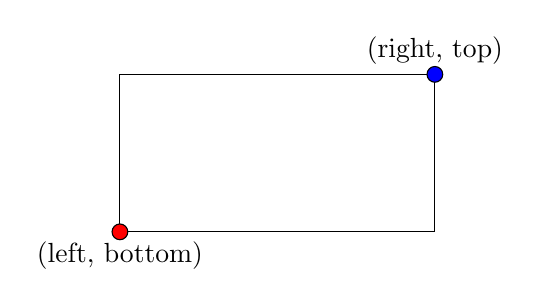
\begin{tikzpicture}
            \draw (0,-8) rectangle (4,-6);
            \draw[fill=red]  (0,-8) circle (0.1);
            \draw[fill=blue] (4,-6) circle (0.1);
            \node at (0,-8.3) {(left, bottom)};
            \node at (4,-5.7) {(right, top)};
	\end{tikzpicture}
\end{frame}

\begin{frame}{Overlaps}
	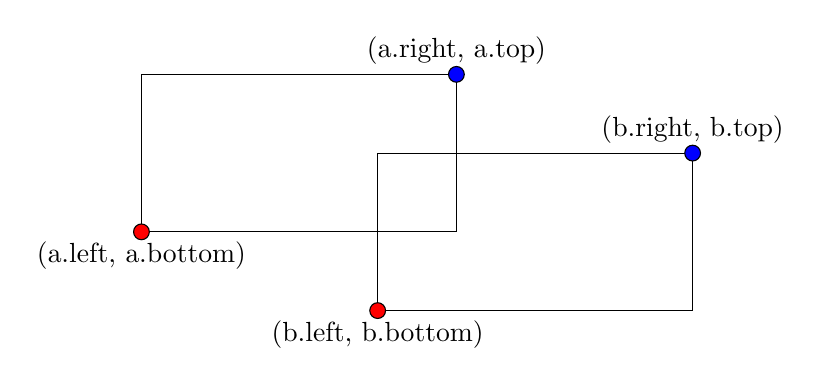
\begin{tikzpicture}
            \draw (0,-8) rectangle (4,-6);
            \draw[fill=red]  (0,-8) circle (0.1);
            \draw[fill=blue] (4,-6) circle (0.1);
            \node at (0,-8.3) {(a.left, a.bottom)};
            \node at (4,-5.7) {(a.right, a.top)};
            
            \draw (3,-9) rectangle (7,-7);
            \draw[fill=red]  (3,-9) circle (0.1);
            \draw[fill=blue] (7,-7) circle (0.1);
            \node at (3,-9.3) {(b.left, b.bottom)};
            \node at (7,-6.7) {(b.right, b.top)};
	\end{tikzpicture}
\end{frame}

\begin{frame}{Reduction from SMT}
        b.left > a.right
    $\parallel$ a.bottom > b.top
\end{frame}

\begin{frame}{Combining in the LSC Semigroup}
    \begin{center}
        overlap + net connect + another constraint
    \end{center}
\end{frame}

\begin{frame}{Stay low}
    \begin{tikzpicture}
        \begin{axis}
          [ xticklabels={,,}
          , yticklabels={,,}
          , scaled ticks=false
          , xmin=0,ymin=0
          , samples=123
          , domain=0:42
          , width=1.1\textwidth,
          , height=0.55\textwidth
          ]
        \addplot[blue] {pow(2,x)} node[above]{};
        \end{axis}
    \end{tikzpicture}
\end{frame}

\begin{frame}{Maximize yield}
	\begin{itemize}
        \setlength\itemsep{1em}
		\item Minimize area of a chip $\rightarrow$ \textit{silicon compiler}
		\item Minimize physical errors $\rightarrow$ \textbf{silicon process}
	\end{itemize}
\end{frame}

\section[Process]{}

\begin{frame}{Features}
	\begin{itemize}
        \setlength\itemsep{1em}
		\item MOSFETs
		\item LDMOSFETs (High voltage) 
		\item BJTs
		\item Zener polysilicon diodes
		\item SONOS flash cells
		\item Polysilicon resistors
		\item Metal caps
	\end{itemize}
\end{frame}

\begin{frame}{Process design considerations}
	\begin{itemize}
		\item Should be portable
		\item Robust
		\item Low amount of layers
		\item KISS (Keep it simple and stupid)
		\item Avoid expensive machines (can be manufactured in a home lab)
	\end{itemize}
\end{frame}

\begin{frame}{Process design considerations}
	\begin{center}
		\includegraphics[height=0.8\textheight]{images/breaking-bad.png}
	\end{center}
\end{frame}

\begin{frame}{Process design considerations}
	\begin{center}
		\includegraphics[height=0.8\textheight]{images/innovation-hub-hamburg.jpg}
	\end{center}
\end{frame}

\begin{frame}{Cross section}
	\begin{center}
		\begin{tikzpicture}[node distance = 3cm, auto, thick,scale=0.2, every node/.style={transform shape}]
			\input{tikz_process_steps/glass.a.tex}
			\node at (5,-0.5) {\textbf{\huge{PMOS}}};
			\node at (13,-0.5) {\textbf{\huge{NMOS}}};
			\node at (22,-0.5) {\textbf{\huge{SONOS flash cell (PMOS)}}};
			\node at (30,-0.5) {\textbf{\huge{NPN BJT}}};
			\node at (38,-0.5) {\textbf{\huge{PNP BJT}}};
			\node at (46,-0.5) {\textbf{\huge{Polysilicon diode}}};
			\node at (52,-0.5) {\textbf{\huge{Polyresistor}}};
		\end{tikzpicture}
	\end{center}
\end{frame}

\begin{frame}{PearlRiver \cjkfont(珠江芯片一号)}
    \begin{center}
        \includegraphics[height=0.8\textheight]{images/Screenshot_20181216_204924.png}
    \end{center}
\end{frame}

\begin{frame}{PearlRiver \cjkfont(珠江芯片一号)}
	\textbf{Fulfills following functions:}
	\begin{itemize}
		\item Debugging
		\item Calibration of new equipment to LibreSilicon
		\item Research of new features
		\item Syncing process features between fabs
	\end{itemize}
\end{frame}

\begin{frame}{Photomask}
	\begin{center}
		\includegraphics[height=0.8\textheight]{images/20181207_113845_Burst01.jpg}
	\end{center}
\end{frame}

\begin{frame}{Photomask}
	\begin{itemize}
		\item Is stepper/aligner brand specific
		\item ASML stepper masks contain 4 layers each
		\item The NFF stepper has a reduction value of 5:1
		\item A 5 micron gate on the mask is 1 micron on the wafer
	\end{itemize}
\end{frame}

\begin{frame}{Photo resist (HKUST)}
	\begin{center}
		\includegraphics[height=0.8\textheight]{images/20181128_154907.jpg}
		\includegraphics[height=0.8\textheight]{images/20181128_154911.jpg}
	\end{center}
\end{frame}

\begin{frame}{Photo resist (HKUST)}
	\textbf{Two types of photo resist:}
	\begin{itemize}
		\item FH 6400L (implantation)
		\item HPR 504 (normal etch)
	\end{itemize}

	\textbf{Factors to consider:}
	\begin{itemize}
		\item Thickness of FH 6400L and implantation energy are interlinked
		\item Thickness of HPR 504 and etching time are interlinked (selectivity)
	\end{itemize}
\end{frame}

\begin{frame}{After exposure}
\begin{center}
\includegraphics[height=0.8\textheight]{images/20181210_125830_Burst01.jpg}
\includegraphics[height=0.8\textheight]{images/20181210_125845.jpg}
\end{center}
\end{frame}

\begin{frame}{Alignment}
\begin{center}
\includegraphics[height=0.8\textheight]{images/20181211_125918.jpg}
\includegraphics[height=0.8\textheight]{images/20181211_161801_Burst01.jpg}
\end{center}
\end{frame}

\begin{frame}{Example: NOR3 ring oscillator}
\begin{center}
	\includegraphics[width=\textwidth]{images/Screenshot_20181219_184458.png}
\end{center}
\end{frame}

\begin{frame}{Example: NOR3 ring oscillator}
\begin{center}
	\textbf{Wells (nwell/pwell):}

	\includegraphics[width=\textwidth]{images/Screenshot_20181221_124540.png}
\end{center}
\end{frame}

\begin{frame}{Example: NOR3 ring oscillator}
\begin{center}
	\textbf{Wells (nwell/pwell):}

	\includegraphics[width=0.25\textwidth]{images/20181214_125705.jpg}
\end{center}
\end{frame}

\begin{frame}{Example: NOR3 ring oscillator}
	\textbf{Recipe for nwell:}
	\begin{itemize}
		\item Coat with implant resist (soft bake 60 seconds, 110\textdegree{}C)
		\item Expose nwell-mask
		\item Puddle develop 69 seconds and hard bake 60 seconds at 120\textdegree{}C
		\item Implant Phosphorus, $2.33 \times 10^{12} cm^{-2}$ @ 70keV
		\item Strip resist with plasma asher or 20 minutes in 120\textdegree{}C hot sulfuric acid
	\end{itemize}
	\textbf{Note:} Alternatively predisposition can be used
\end{frame}

\begin{frame}{Example: NOR3 ring oscillator}
	\textbf{Recipe for pwell:}
	\begin{itemize}
		\item Coat with implant resist (soft bake 60 seconds, 110\textdegree{}C)
		\item Expose pwell-mask
		\item Puddle develop 69 seconds and hard bake 60 seconds at 120\textdegree{}C
		\item Implant Boron, $1.93 \times 10^{12} cm^{-2}$ @ 40keV
		\item Strip resist with plasma asher or 20 minutes in 120\textdegree{}C hot sulfuric acid
		\item Diffuse both wells together for 4 hours at 1050\textdegree{}C in inert atmosphere ($N_2$) 
	\end{itemize}
	\textbf{Note:} Alternatively predisposition can be used
\end{frame}

\begin{frame}{The Fick's equation}
\begin{center}
	\begingroup
	\huge
	$\frac{\partial N}{\partial t} = D \cdot \frac{\partial^2 N}{\partial x^2}$
	\endgroup
\end{center}
\end{frame}

\definecolor{LightCyan}{rgb}{0.88,1,1}

\begin{frame}{The Fick's equation}
\begin{center}
	$x_l(t) = 2 \cdot \sqrt{D_e \cdot t} = 2 \cdot \sqrt{D_0 \cdot \exp\left(-\frac{E_a}{k \cdot T}\right) \cdot t}$ \\
	\begin{tabular}{|c|c|c|}
		\hline
		\textbf{Element} &
		$D_0$ $\left[\frac{cm^2}{s}\right]$ &
		$E_a$ $\left[eV\right]$ \\
		\hline
		\rowcolor{LightCyan}
		P &
		10.50 &
		3.69 \\
		\hline
		As &
		0.32 &
		3.56 \\
		\hline
		Sb &
		5.60 &
		3.95 \\
		\hline
		\rowcolor{LightCyan}
		B &
		10.50 &
		3.69 \\
		\hline
		Al &
		8.00 &
		3.47 \\
		\hline
		Ga &
		3.60 &
		3.51 \\
		\hline
		Cu &
		0.0025 &
		0.65 \\
		\hline
	\end{tabular}
\end{center}
\end{frame}

\begin{frame}{The Fick's equation}
	\begin{center}
		\begingroup
		\huge
		$N(x,t)=\frac{Q}{\sqrt{\pi \cdot D_e \cdot t}} \cdot \exp\left(\frac{-x^2}{4 \cdot D_e \cdot t}\right)$
		\endgroup
	\end{center}
\end{frame}

\begin{frame}{The Fick's equation}
	\begin{center}
		For the concentration within the channel may $x=0$

		This results in the concentration at the surface (around 100nm deep $\ll$ 2 microns)

		$ N = \frac{Q}{\sqrt{\pi \cdot D_e \cdot t}} $

		Or the implant dosage:

		$ Q = N \cdot \sqrt{\pi \cdot D_e \cdot t} $
	\end{center}
\end{frame}

\begin{frame}{The Fick's equation}
	\begin{center}
		Fixed source diffusion:

		$ x_j = 2 \cdot\sqrt{D \cdot t \cdot \ln\left(\frac{N_0}{N_B}\right)} $

		\includegraphics[width=0.25\textwidth]{images/well_formation1.png}
		\includegraphics[width=0.25\textwidth]{images/well_formation2.png}
	\end{center}
\end{frame}

\begin{frame}{Threshold calculation}
	\begin{center}
		\textbf{PMOS}

		\begin{equation}
			\left| \phi_F \right| = V_T \ln\frac{N_d}{n_i}
		\end{equation}

		\begin{equation}
			V_T
			=
			V_{FB}
			-
			2 \cdot \left| \phi_F \right|
			-
			\frac{
			\sqrt{2 \cdot \epsilon_s \cdot 2 \cdot \left| \phi_F \right| \cdot q \cdot N_d }
			}{C_{ox}}
		\end{equation}

		\begin{equation}
			V_T = V_FB - abs{2 \phi_F}
		\end{equation}
	\end{center}
\end{frame}

\begin{frame}{Threshold calculation}
	\begin{center}
		\textbf{NMOS}

		\begin{equation}
			\phi_F = V_T \ln\frac{N_a}{n_i}
		\end{equation}

		\begin{equation}
			V_T
			=
			V_{FB}
			-
			2 \cdot \left| \phi_F \right|
			-
			\frac{
			\sqrt{2 \cdot \epsilon_s \cdot 2 \cdot \left| \phi_F \right| \cdot q \cdot N_d }
			}{C_{ox}}
		\end{equation}

		\begin{equation}
			V_T = V_FB - abs{2 \phi_F}
		\end{equation}
	\end{center}
\end{frame}

\begin{frame}{Example: NOR3 ring oscillator}
	\begin{center}
		\textbf{Isolation (STI):}

		\includegraphics[width=\textwidth]{images/Screenshot_20181220_164222.png}
	\end{center}
\end{frame}

\begin{frame}{Example: NOR3 ring oscillator}
\begin{center}
	\textbf{Isolation (STI):}

	\includegraphics[width=0.25\textwidth]{images/20181219_125354_Burst01.jpg}
	\includegraphics[width=0.25\textwidth]{images/20181219_125758.jpg}
\end{center}
\end{frame}

\begin{frame}{Example: NOR3 ring oscillator}
	\textbf{Recipe for STI:}
	\begin{itemize}
		\item\textbf{Dry}
		\begin{itemize}
			\item Plasma etching recipes are machine specific
			\item Variate the cycles for your recipe to match 2 microns
		\end{itemize}
		\item\textbf{Wet}
		\begin{itemize}
			\item Take TMAH: $ N ( CH _3 ) _4 ^{+} OH ^{−}$ (Tetramethylammonium hydroxide)
			\item Dilute with deionized water with DI:TMAH (3:1)
			\item Heat TMAH (25\%) to 80\textdegree{}C
			\item Dip wafer into the solution for around 6 minutes and 15 seconds (320nm/min, 2 microns)
		\end{itemize}
	\end{itemize}
\end{frame}

\begin{frame}{Example: NOR3 ring oscillator}
\begin{center}
	\textbf{Metal interconnect (metal1):}

	\includegraphics[width=\textwidth]{images/Screenshot_20181219_184526.png}
\end{center}
\end{frame}

\begin{frame}{Example: NOR3 ring oscillator}
\begin{center}
	\textbf{Metal interconnect (metal1):}

	\includegraphics[width=0.25\textwidth]{images/20181218_115931.jpg}
	\includegraphics[width=0.25\textwidth]{images/20181218_161016.jpg}
\end{center}
\end{frame}

\begin{frame}{Example: NOR3 ring oscillator}
	\textbf{Recipe for metal interconnects:}

	\begin{itemize}
		\item Make a vacuum (low pressure)
		\item Deposit 100nm Aluminum
		\item Deposit 30nm Titanium over the Aluminum
		\item Take out of vacuum
		\item Dip into HF:DI (1:10) water solution for a few seconds until Titanium is gone
		\item Dip into FeCl3 or other suitable Aluminum etchant for around 30 seconds until Aluminum is gone
	\end{itemize}
	
\end{frame}

\end{document}
